\documentclass[12pt,a4paper]{article}

\usepackage[T2A]{fontenc}
\usepackage[utf8]{inputenc}
\usepackage[russian]{babel}
\usepackage{amsmath,amssymb}
\usepackage{graphicx}
\usepackage{booktabs}
\usepackage{tabularx}
\usepackage{makecell}
\usepackage{float}
\usepackage{caption}
\usepackage{subcaption}
\usepackage{enumitem}
\usepackage{xurl}
\usepackage{hyperref}
\usepackage{ragged2e}
\usepackage{geometry}
\usepackage{microtype}

\geometry{
    left=25mm,
    right=20mm,
    top=22mm,
    bottom=24mm
}

\hypersetup{
    colorlinks=true,
    linkcolor=black,
    citecolor=black,
    urlcolor=black
}

\setlength{\parindent}{1.25cm}
\setlength{\parskip}{0pt}
\renewcommand{\arraystretch}{1.18}
\captionsetup{font=small,labelfont=bf}
\Urlmuskip=0mu plus 2mu
\emergencystretch=2em

\newcommand{\CodeRepository}{\url{https://github.com/Vitamj/funkan-cases-3-7}}
\newcommand{\R}{\mathbb{R}}
\newcommand{\one}{\mathbf{1}}
\newcommand{\eps}{\varepsilon}

\begin{document}

\begin{titlepage}
    \thispagestyle{empty}
    \begin{center}
        Университет ИТМО\\
        Факультет информационных технологий и программирования\\[2.2cm]

        {\Large Лабораторная работа по функциональному анализу}\\[0.5cm]
        {\LARGE\bfseries Спектральное восстановление геометрии\\
        и аддитивная аппроксимация функций}\\[0.4cm]
        {\large Кейсы 3 и 7}\\[2cm]
    \end{center}

    \begin{flushright}
        Выполнила: Мижа Виктория\\
        Группа: J3213\\
        Формат выполнения: индивидуально\\
        Выбранные кейсы: 3 и 7\\
    \end{flushright}

    \vfill

    \begin{center}
        Санкт-Петербург\\
        2026
    \end{center}
\end{titlepage}

\setcounter{page}{1}
\tableofcontents
\newpage

\section*{Аннотация}
\addcontentsline{toc}{section}{Аннотация}

В работе рассматриваются две задачи, в которых функционально-аналитические идеи
переходят в вычислительные методы. В кейсе 3 исследуется матрица попарных
расстояний: проверяются ее метрические свойства, выводится формула двойного
центрирования, строится матрица Грама и восстанавливается конфигурация точек.
В кейсе 7 строится аддитивная регрессионная модель, в которой функция многих
переменных приближается суммой одномерных функций, заданных в конечном базисе.

Основной результат первой части: минимальная размерность точного евклидова
вложения определяется числом положительных собственных значений матрицы Грама.
Основной результат второй части: аддитивная модель хорошо работает на данных,
где зависимость действительно является суммой одномерных эффектов, но теряет
качество при наличии взаимодействий между признаками.

\section{Постановка задачи}

\subsection{Кейс 3: изометрия и матрица расстояний}

Пусть задано конечное множество объектов
\[
    X=\{x_1,\ldots,x_n\}
\]
и матрица попарных расстояний
\[
    D=(d_{i,j})_{i,j=1}^{n}, \qquad d_{i,j}=d(x_i,x_j).
\]
Требуется определить, можно ли найти точки
\[
    y_1,\ldots,y_n\in\R^m
\]
такие, что
\[
    \|y_i-y_j\|=d_{i,j}, \qquad i,j=1,\ldots,n.
\]
Если такие точки существуют, отображение \(x_i\mapsto y_i\) является
изометрическим вложением конечного метрического пространства в евклидово
пространство.

В рамках исследования нужно:
\begin{enumerate}[label=\arabic*)]
    \item проверить базовые свойства матрицы расстояний;
    \item вывести и применить формулу двойного центрирования;
    \item построить матрицу Грама и исследовать ее спектр;
    \item восстановить координаты точек в полной и низкой размерности;
    \item оценить ошибку восстановления расстояний;
    \item проверить устойчивость результата при добавлении шума.
\end{enumerate}

\subsection{Кейс 7: аддитивная модель}

Рассматривается регрессионная задача
\[
    y=f(x_1,\ldots,x_p)+\eps,\qquad x_j\in[0,1],
\]
где \(\eps\) --- случайный шум. Вместо полной многомерной аппроксимации
используется аддитивная модель
\[
    \widehat f(x)=\beta_0+\sum\limits_{j=1}^{p}g_j(x_j).
\]
Каждая одномерная компонента представляется в конечном базисе:
\[
    g_j(t)=\sum\limits_{m=1}^{M}a_{j,m}\psi_m(t).
\]
После построения блочной матрицы признаков задача становится линейной по
параметрам.

В рамках исследования нужно:
\begin{enumerate}[label=\arabic*)]
    \item построить обучающую и тестовую выборки;
    \item выбрать базис для функций \(g_j\);
    \item оценить параметры аддитивной модели;
    \item выполнить центрирование компонент;
    \item сравнить аддитивную модель с линейной и полной нелинейной моделями;
    \item исследовать влияние числа базисных функций;
    \item проверить качество на неаддитивных данных.
\end{enumerate}

\section{Обозначения}

В отчете используются следующие обозначения:
\begin{itemize}
    \item \(n\) --- число объектов в кейсе 3;
    \item \(D=(d_{i,j})\) --- матрица расстояний;
    \item \(D^{(2)}=(d_{i,j}^2)\) --- матрица квадратов расстояний;
    \item \(\one=(1,\ldots,1)^{T}\);
    \item \(J=I-\frac{1}{n}\one\one^{T}\) --- матрица центрирования;
    \item \(B=(b_{i,j})\) --- матрица Грама центрированной конфигурации;
    \item \(r\) --- число положительных собственных значений матрицы \(B\);
    \item \(p\) --- число признаков в регрессионной задаче;
    \item \(M\) --- число базисных функций на один признак;
    \item \(\ell\) --- объем обучающей выборки;
    \item \(\eps\) --- случайный шум;
    \item \(\lambda\) --- коэффициент ridge-регуляризации.
\end{itemize}

Парные индексы записываются через запятую: \(d_{i,j}\), \(b_{i,j}\),
\(x_{i,j}\). Это делает формулы с двойными индексами более читаемыми.

\section{Метод для кейса 3}

\subsection{Проверка метрических свойств}

Матрица расстояний должна удовлетворять следующим условиям:
\[
    d_{i,i}=0,\qquad
    d_{i,j}=d_{j,i},\qquad
    d_{i,j}\ge 0,
\]
а также неравенству треугольника
\[
    d_{i,j}\le d_{i,k}+d_{k,j},
    \qquad i,j,k=1,\ldots,n.
\]
Эти свойства необходимы для метрической матрицы расстояний, но сами по себе
еще не гарантируют евклидову реализуемость. Поэтому следующим шагом матрица
расстояний переводится в матрицу Грама.

\subsection{Вывод формулы двойного центрирования}

Пусть \(B=(b_{i,j})\) --- матрица Грама центрированной конфигурации:
\[
    b_{i,j}=\langle y_i,y_j\rangle,\qquad
    \sum\limits_{i=1}^{n}y_i=0.
\]
Тогда квадрат расстояния между двумя точками выражается через элементы матрицы
Грама:
\[
    d_{i,j}^{2}
    =\|y_i-y_j\|^2
    =b_{i,i}+b_{j,j}-2b_{i,j}.
\]
Обозначим \(q_{i,j}=d_{i,j}^{2}\). Так как конфигурация центрирована, суммы
строк и столбцов матрицы \(B\) равны нулю:
\[
    \sum\limits_{j=1}^{n}b_{i,j}=0,
    \qquad
    \sum\limits_{i=1}^{n}b_{i,j}=0.
\]
Усредняя \(q_{i,j}\) по строкам, столбцам и всей матрице, получаем
\[
    \overline q_{i,\cdot}=b_{i,i}+\frac{\operatorname{tr}B}{n},
    \qquad
    \overline q_{\cdot,j}=b_{j,j}+\frac{\operatorname{tr}B}{n},
    \qquad
    \overline q_{\cdot,\cdot}=2\frac{\operatorname{tr}B}{n}.
\]
Следовательно,
\[
    b_{i,j}
    =
    -\frac{1}{2}
    \left(
        q_{i,j}
        -\overline q_{i,\cdot}
        -\overline q_{\cdot,j}
        +\overline q_{\cdot,\cdot}
    \right).
\]
В матричной форме это дает формулу двойного центрирования:
\[
    B=-\frac{1}{2}JD^{(2)}J,
    \qquad
    J=I-\frac{1}{n}\one\one^{T}.
\]
Центрирование устраняет неопределенность, связанную с переносом всей
конфигурации: если ко всем точкам прибавить один и тот же вектор, расстояния
между точками не изменятся.

\subsection{Спектральное восстановление координат}

Если расстояния евклидовы, то матрица \(B\) должна быть положительно
полуопределенной. Ее спектральное разложение имеет вид
\[
    B=U\Lambda U^{T}.
\]
Пусть \(\Lambda_r\) содержит положительные собственные значения, а \(U_r\) ---
соответствующие собственные векторы. Тогда координаты можно взять в виде
\[
    Y=U_r\Lambda_r^{1/2}.
\]
Действительно,
\[
    YY^{T}
    =
    U_r\Lambda_r^{1/2}\Lambda_r^{1/2}U_r^{T}
    =
    U_r\Lambda_rU_r^{T}
    =
    B_r.
\]
Если используются все положительные собственные значения и отрицательных
собственных значений нет, восстановление является точным с точностью до
сдвига, поворота и отражения. Если часть положительного спектра отброшена,
получается приближенное низкоразмерное вложение.

\subsection{Ошибки восстановления}

Для восстановленных координат строится матрица расстояний \(\widehat D\). Далее
используются три величины:
\[
    E_{\max}=\max\limits_{i,j}|d_{i,j}-\widehat d_{i,j}|,
\]
\[
    E_F=\|D-\widehat D\|_F,
\]
\[
    E_{\operatorname{rel}}
    =
    \frac{\|D-\widehat D\|_F}{\|D\|_F}.
\]
Здесь \(E_{\max}\) и \(E_F\) имеют размерность расстояния, а
\(E_{\operatorname{rel}}\) является безразмерной относительной ошибкой.

\section{Результаты моделирования для кейса 3}

В эксперименте сгенерированы \(45\) точек в \(\mathbb R^3\) на слегка
зашумленной спирали. По исходным координатам построена точная матрица
евклидовых расстояний. Результаты проверки базовых метрических свойств
приведены в таблице~\ref{tab:metric-check}.

\begin{table}[H]
    \centering
    \small
    \caption{Проверка базовых метрических свойств точной матрицы расстояний.}
    \label{tab:metric-check}
    \begin{tabularx}{\textwidth}{c c c c c c}
        \toprule
        \(n\) &
        \makecell{max диаг.\\(расст.)} &
        \makecell{max асим.\\(расст.)} &
        \makecell{отриц.\\(шт.)} &
        \makecell{проверено\\троек (шт.)} &
        \makecell{нарушений\\треуг. (шт.)} \\
        \midrule
        45 & 0.0000 & 0.0000 & 0 & 91125 & 0 \\
        \bottomrule
    \end{tabularx}
\end{table}

Матрица расстояний проходит базовую метрическую проверку. Далее применяется
двойное центрирование и строится спектр матрицы Грама.

\begin{figure}[H]
    \centering
    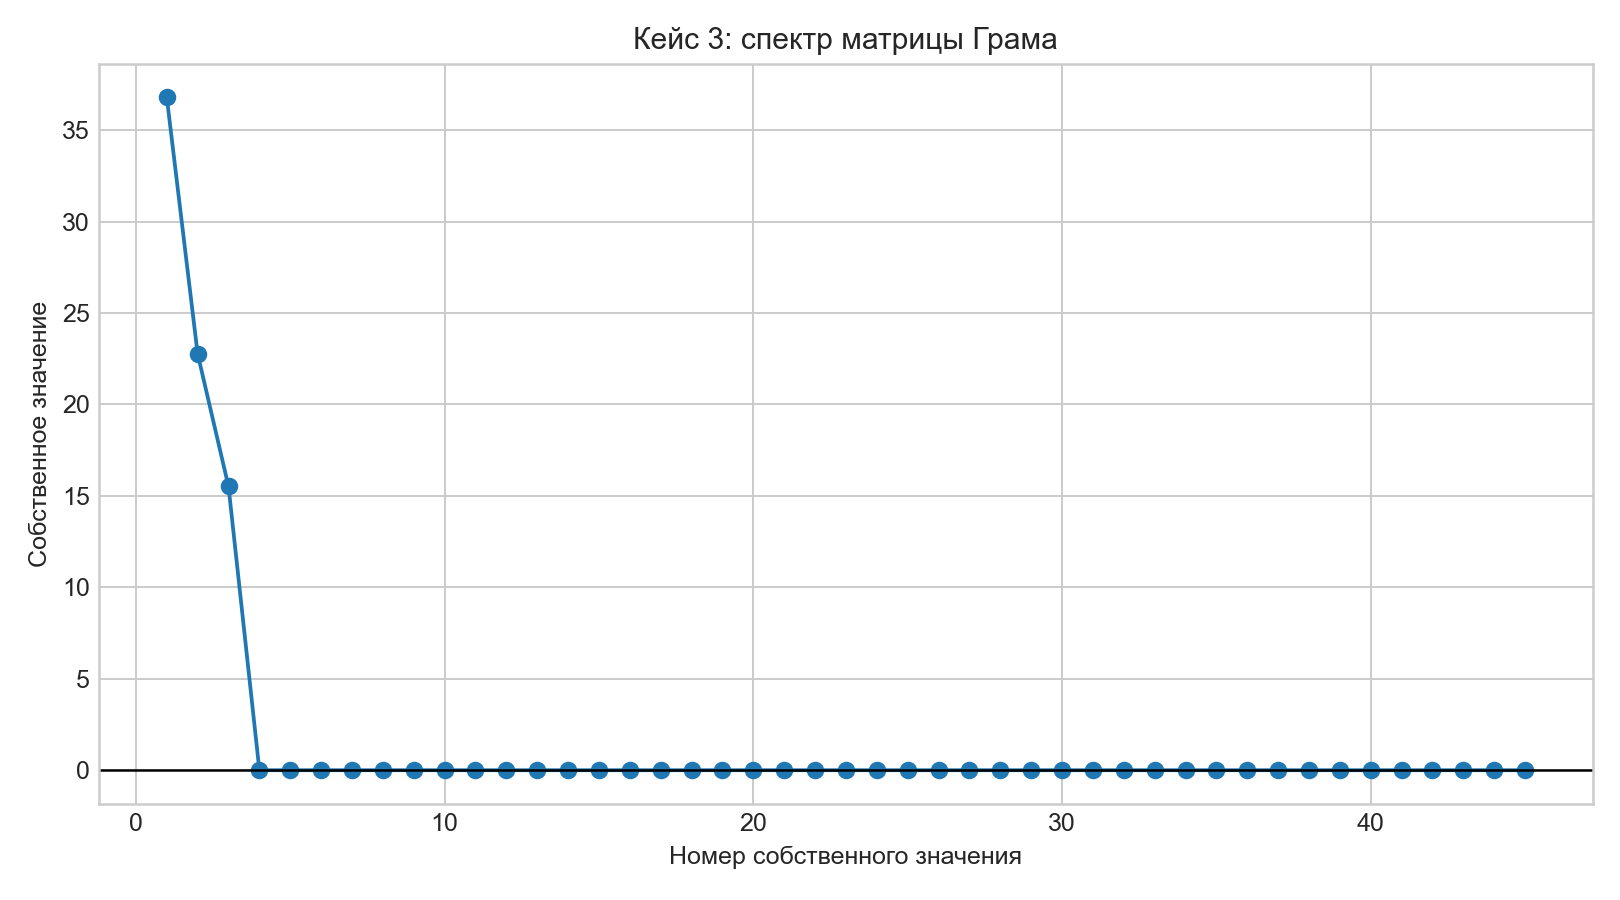
\includegraphics[width=0.82\textwidth]{figures/case3_gram_spectrum.png}
    \caption{Спектр матрицы Грама. Три положительных собственных значения
    задают минимальную размерность точного евклидова вложения.}
    \label{fig:case3-spectrum}
\end{figure}

Из рисунка~\ref{fig:case3-spectrum} видно, что существенная положительная часть
спектра состоит из трех собственных значений. Следовательно, минимальная
размерность точного вложения равна \(3\), что совпадает с размерностью
исходных синтетических точек.

\begin{figure}[H]
    \centering
    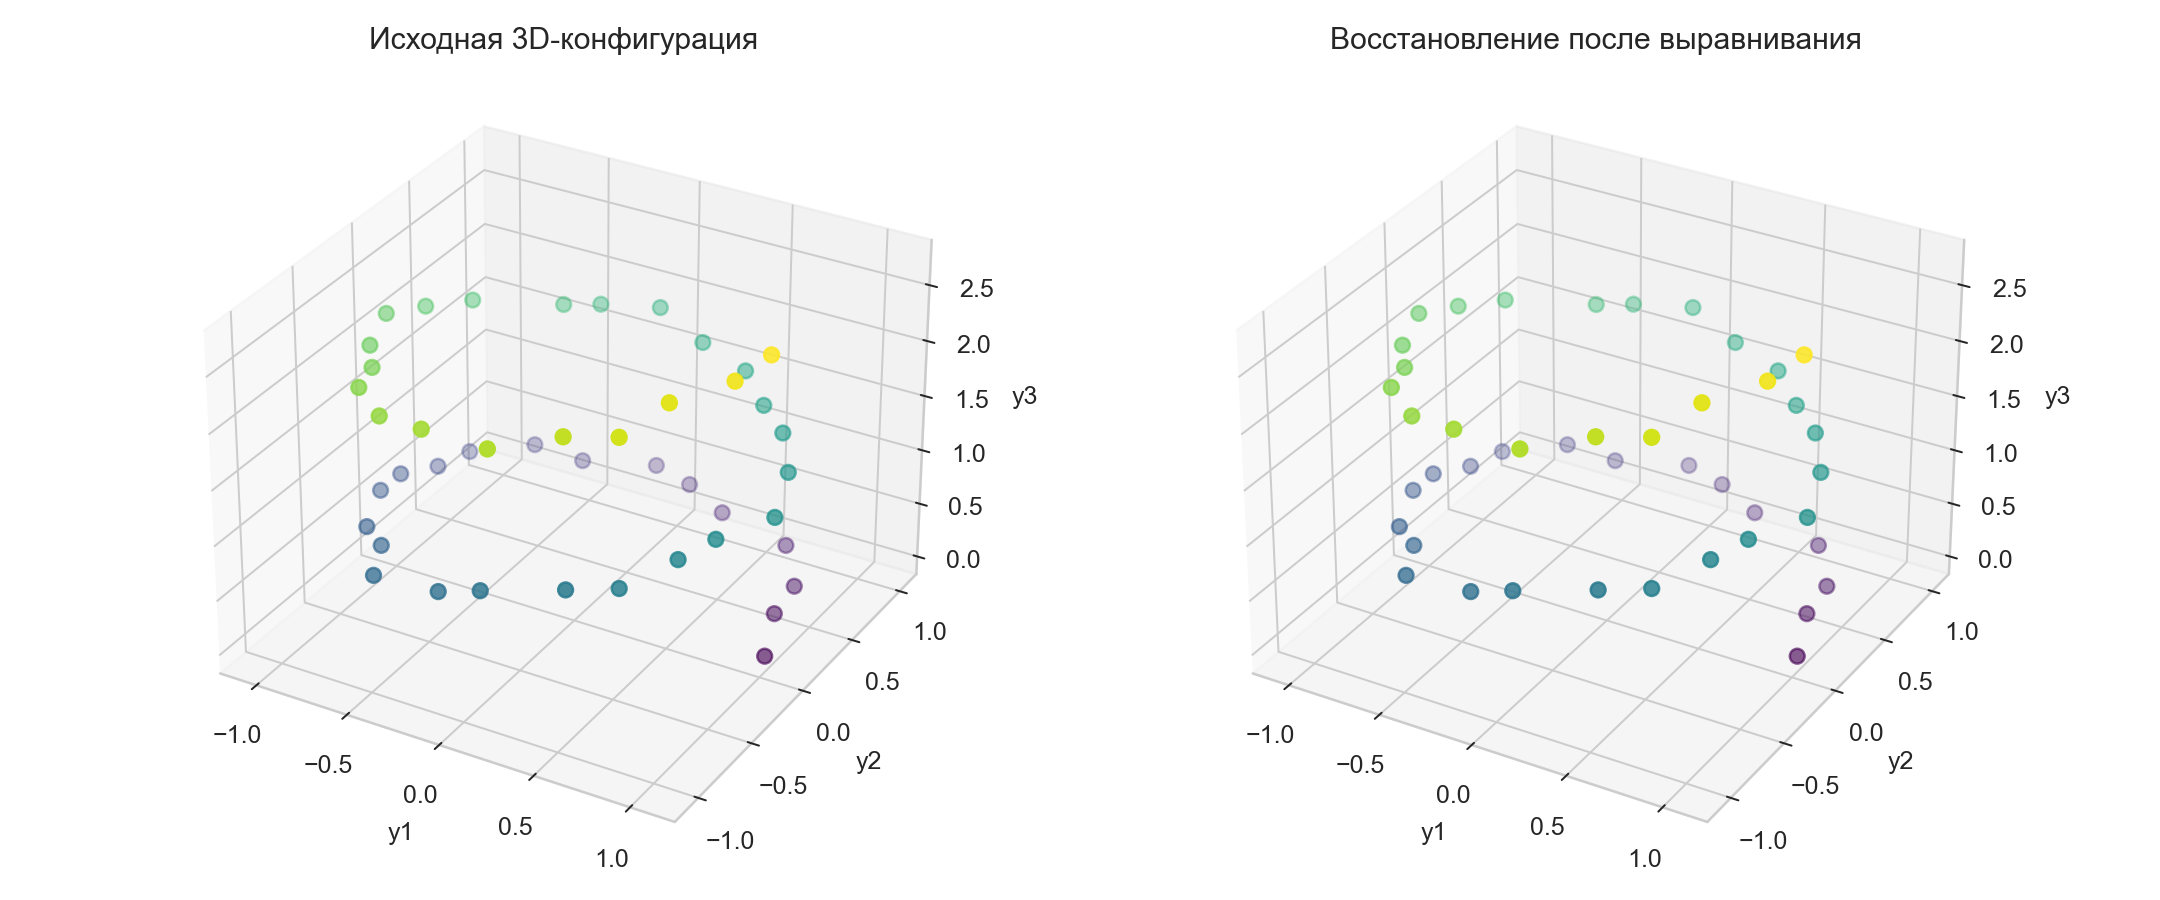
\includegraphics[width=\textwidth]{figures/case3_true_vs_recovered_3d.png}
    \caption{Исходная и восстановленная трехмерные конфигурации после
    выравнивания с точностью до движения пространства.}
    \label{fig:case3-3d}
\end{figure}

На рисунке~\ref{fig:case3-3d} восстановленная конфигурация совпадает с
исходной после выравнивания. Это ожидаемо: матрица расстояний не фиксирует
абсолютное положение и ориентацию точек.

\begin{table}[H]
    \centering
    \small
    \caption{Ошибка восстановления расстояний при разных размерностях вложения.}
    \label{tab:case3-dim}
    \begin{tabularx}{0.82\textwidth}{c c c c}
        \toprule
        \(m\) &
        \makecell{\(E_{\max}\)\\(расст.)} &
        \makecell{\(E_F\)\\(расст.)} &
        \makecell{\(E_{\operatorname{rel}}\)\\(безразм.)} \\
        \midrule
        1 & 2.0959 & 38.3374 & 0.4664 \\
        2 & 1.7907 & 17.8419 & 0.2171 \\
        3 & \(3.11\cdot10^{-15}\) & \(3.77\cdot10^{-14}\) & \(4.58\cdot10^{-16}\) \\
        \bottomrule
    \end{tabularx}
\end{table}

Таблица~\ref{tab:case3-dim} показывает, что при \(m=1\) и \(m=2\) расстояния
искажаются, поскольку часть положительного спектра отброшена. При \(m=3\)
ошибка становится численно нулевой.

\begin{figure}[H]
    \centering
    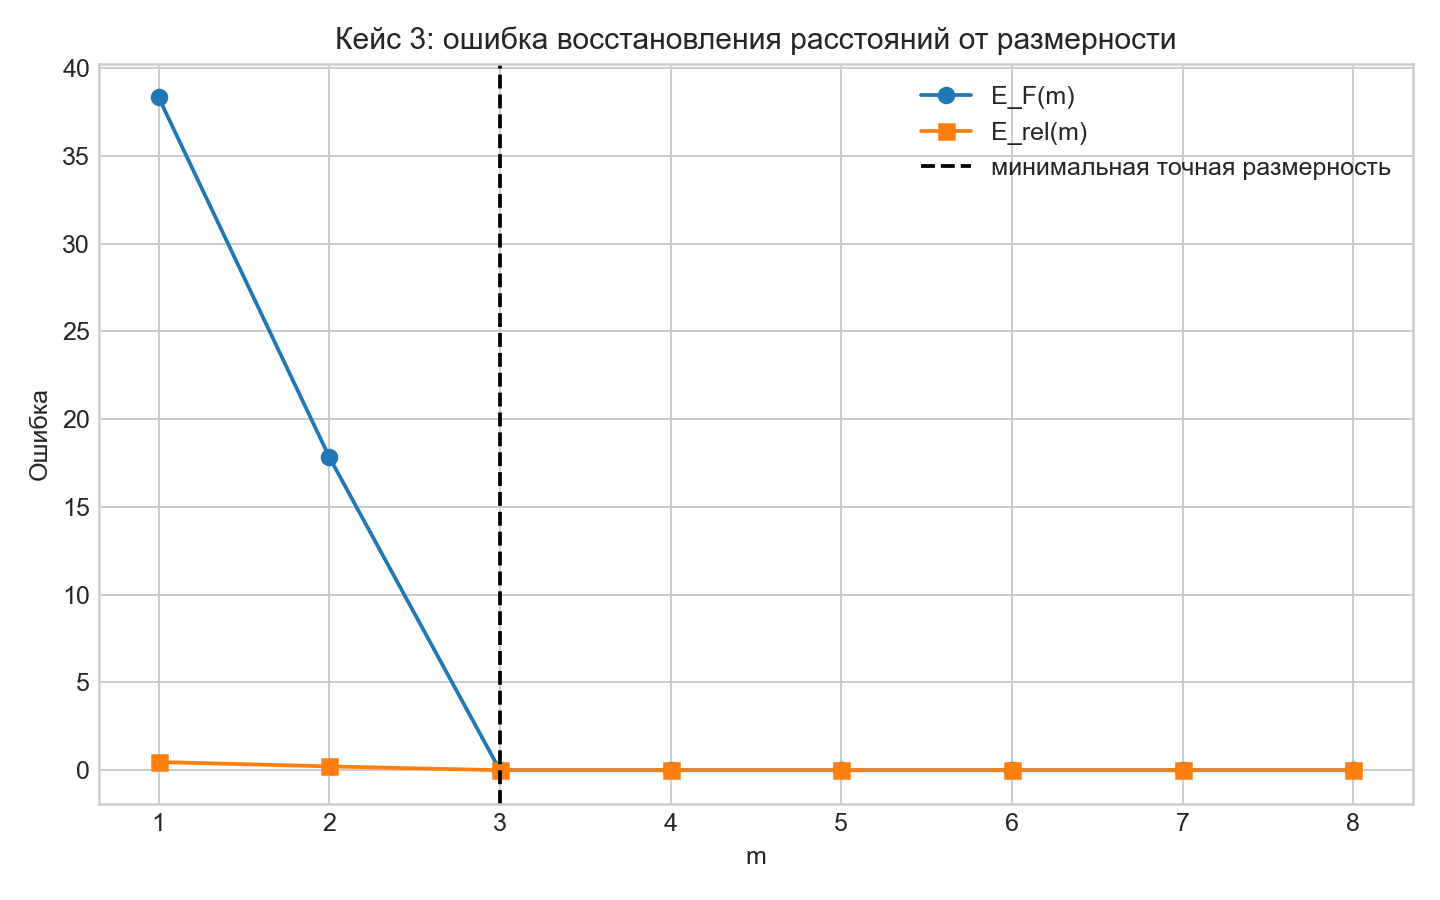
\includegraphics[width=0.82\textwidth]{figures/case3_dimension_error_curve.png}
    \caption{Зависимость ошибки восстановления от размерности вложения.}
    \label{fig:case3-dim-error}
\end{figure}

\begin{figure}[H]
    \centering
    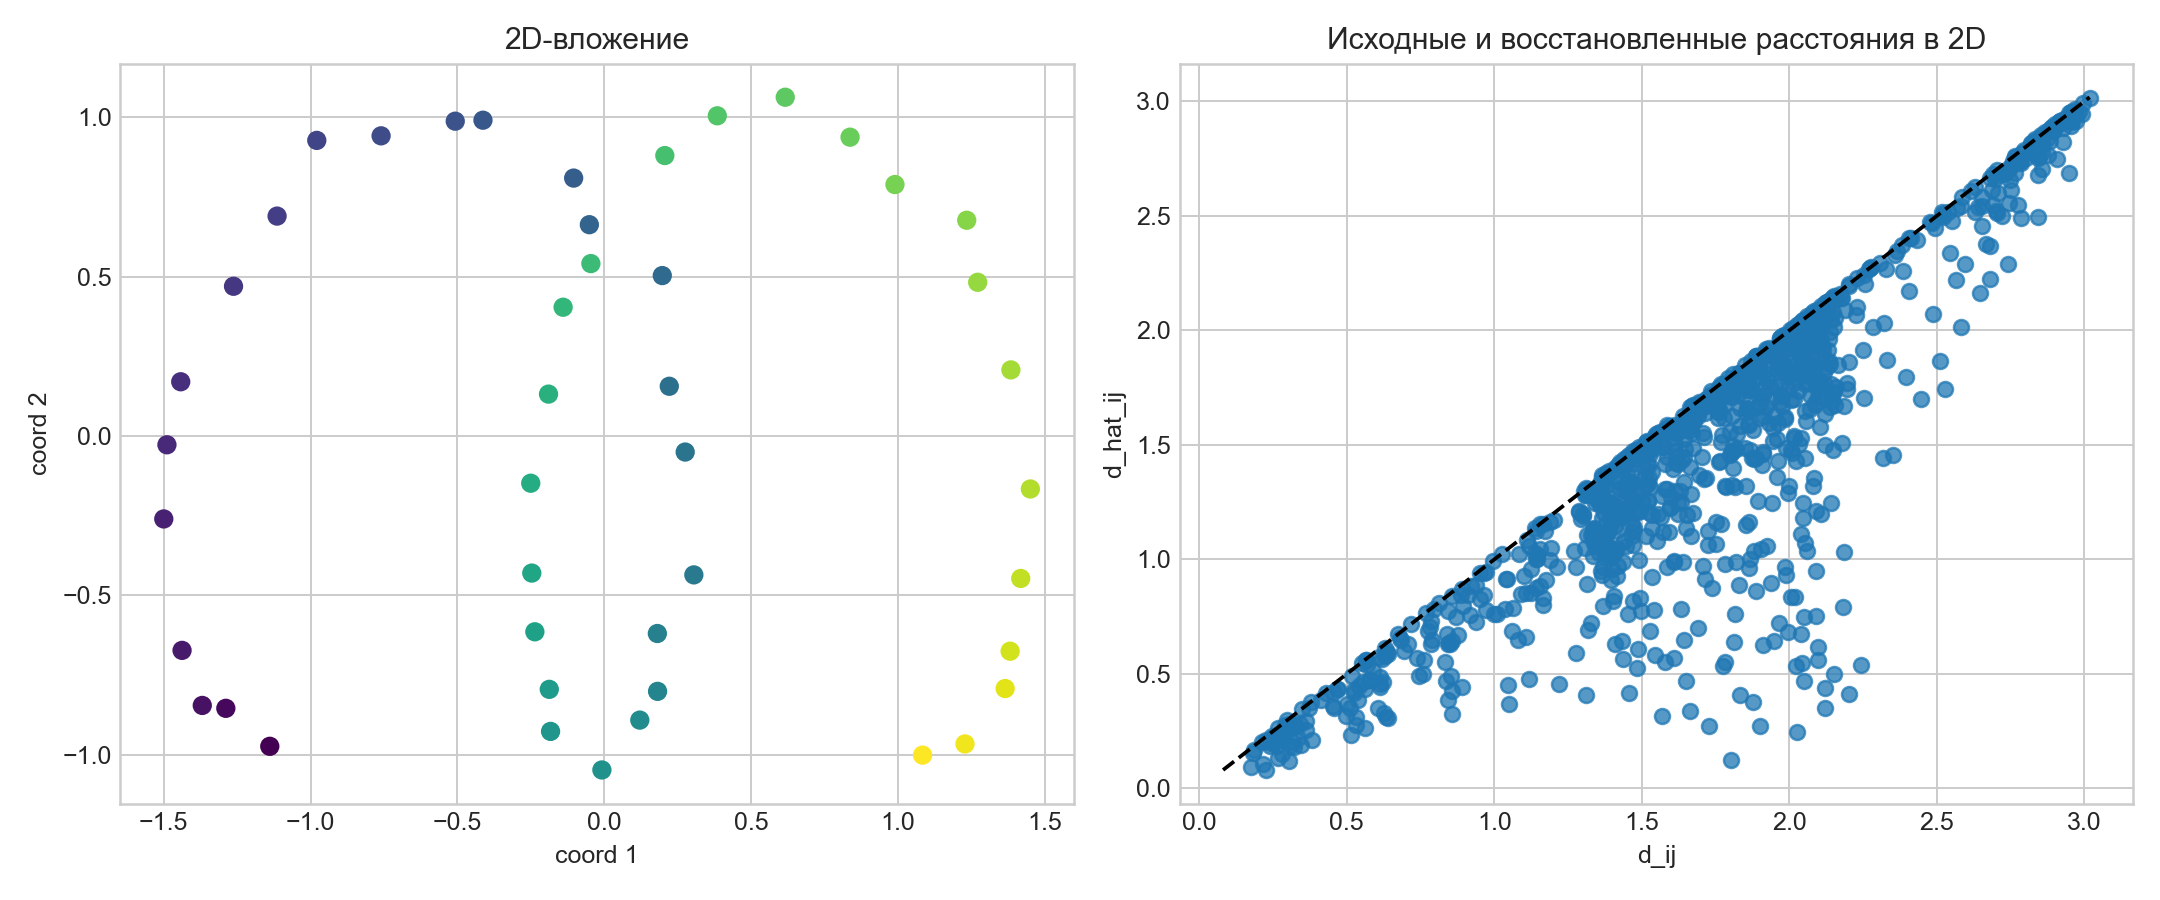
\includegraphics[width=\textwidth]{figures/case3_2d_embedding_and_distances.png}
    \caption{Двумерное вложение и диаграмма ``исходные расстояния ---
    восстановленные расстояния''.}
    \label{fig:case3-2d}
\end{figure}

Двумерное вложение на рисунке~\ref{fig:case3-2d} полезно для визуализации, но
не является изометрическим: точки на диаграмме расстояний заметно отклоняются
от диагонали.

Для проверки устойчивости к шуму строилась матрица
\[
    D^{(\eps)}
    =
    D+\eps\,\operatorname{median}(D)R,
\]
где \(R\) --- симметричная матрица с нулевой диагональю. Параметр \(\eps\)
является безразмерным уровнем шума.

\begin{table}[H]
    \centering
    \small
    \caption{Влияние шума на метрические свойства и ошибку восстановления.}
    \label{tab:case3-noise}
    \begin{tabularx}{\textwidth}{c c c c}
        \toprule
        \(\eps\) &
        \makecell{доля нарушений\\треугольника} &
        \makecell{отрицательных\\собств. знач. (шт.)} &
        \makecell{\(E_{\operatorname{rel}}\)\\(безразм.)} \\
        \midrule
        0.00 & 0.0000 & 0  & 0.0000 \\
        0.05 & 0.0030 & 20 & 0.0758 \\
        0.10 & 0.0078 & 20 & 0.1362 \\
        0.20 & 0.0200 & 20 & 0.2415 \\
        \bottomrule
    \end{tabularx}
\end{table}

\begin{figure}[H]
    \centering
    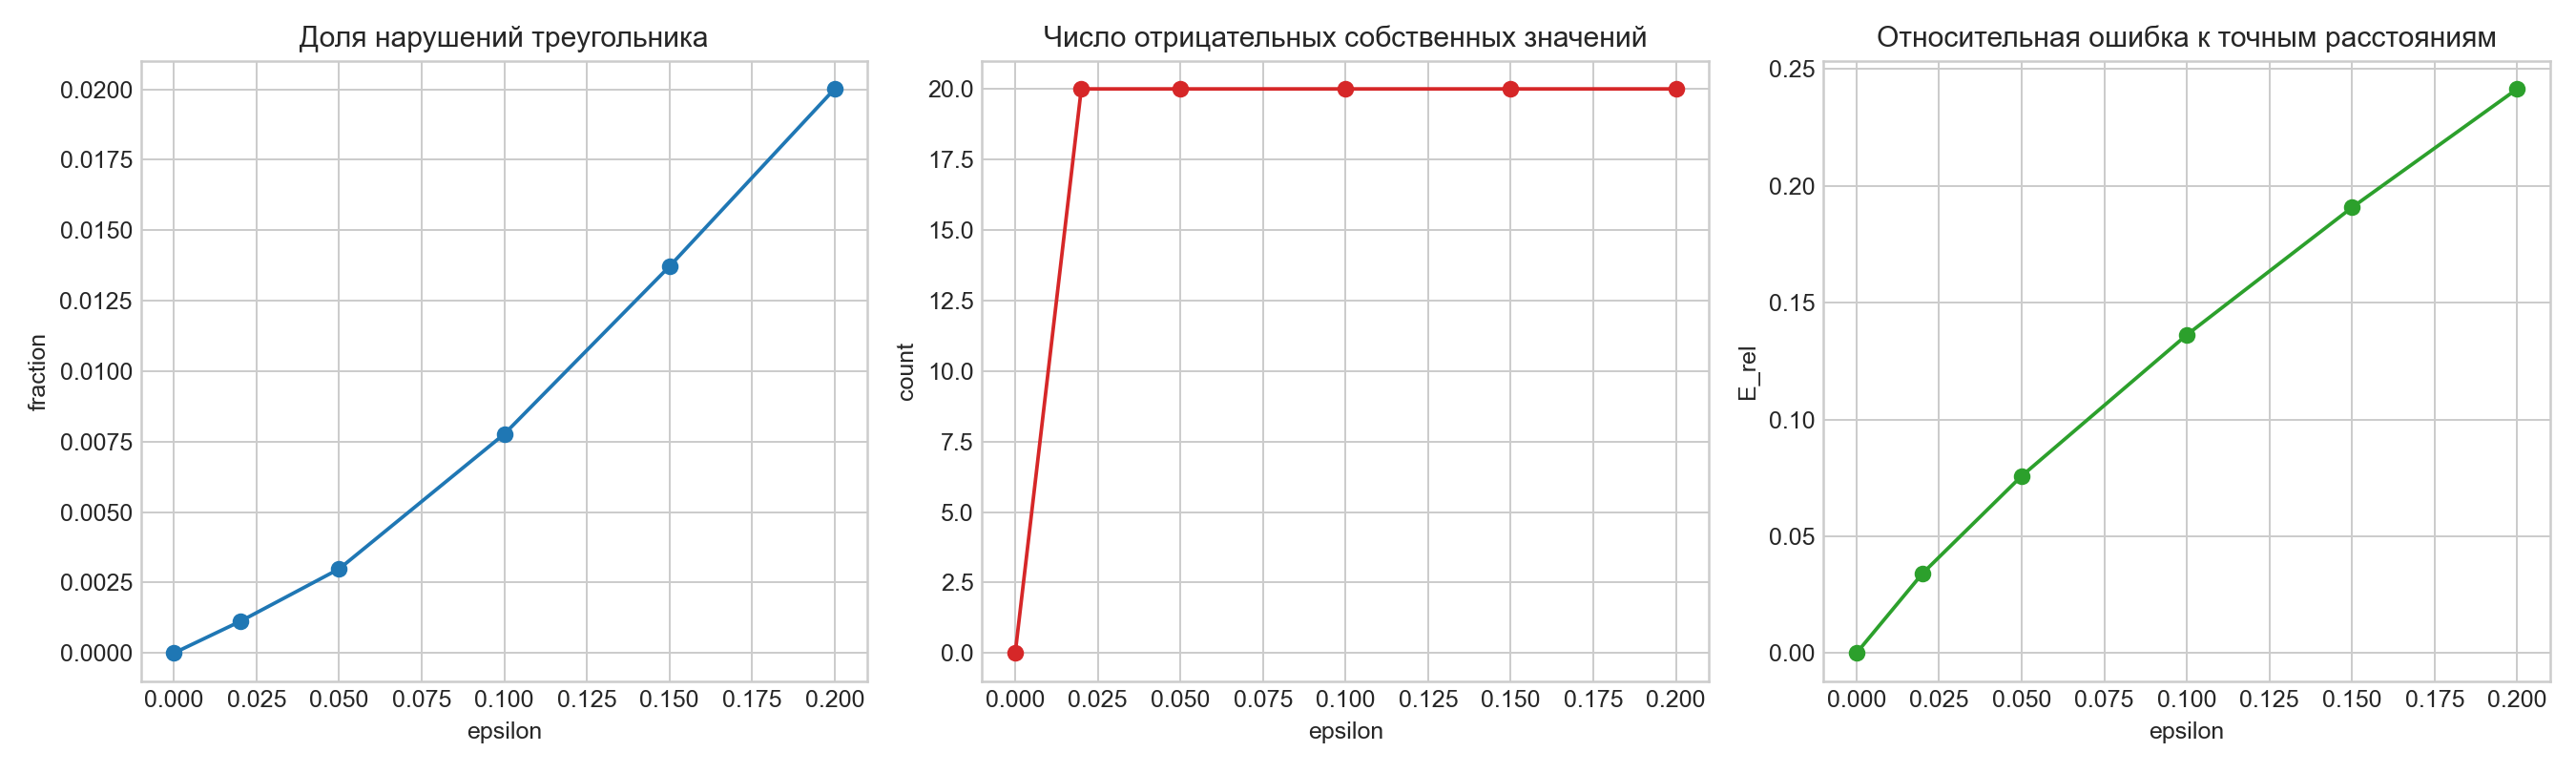
\includegraphics[width=\textwidth]{figures/case3_noise_stability.png}
    \caption{Устойчивость восстановления при добавлении шума.}
    \label{fig:case3-noise}
\end{figure}

При росте \(\eps\) появляются нарушения неравенства треугольника, отрицательные
собственные значения матрицы Грама и рост относительной ошибки. Следовательно,
спектр матрицы Грама является не только инструментом восстановления координат,
но и диагностикой качества исходной матрицы расстояний.

\section{Метод для кейса 7}

\subsection{Базисное разложение}

Аддитивная модель имеет вид
\[
    \widehat f(x)
    =
    \beta_0+\sum\limits_{j=1}^{p}g_j(x_j).
\]
В работе используется полиномиальный базис без отдельной константы:
\[
    \psi_m(t)=t^m,\qquad m=1,\ldots,M.
\]
Тогда
\[
    g_j(t)=\sum\limits_{m=1}^{M}a_{j,m}\psi_m(t),
\]
а для объекта \(x_i\) строка блочной матрицы признаков имеет вид
\[
    z_i=
    \bigl(
    1,\psi_1(x_{i,1}),\ldots,\psi_M(x_{i,1}),
    \ldots,
    \psi_1(x_{i,p}),\ldots,\psi_M(x_{i,p})
    \bigr).
\]
Модель записывается как
\[
    \widehat y_i=z_i^{T}\theta.
\]

\subsection{Оценивание параметров и центрирование}

Параметры оцениваются методом наименьших квадратов с малой
ridge-регуляризацией:
\[
    \widehat\theta
    =
    (Z^{T}Z+\lambda P)^{-1}Z^{T}y.
\]
Матрица \(P\) выбрана так, что свободный член \(\beta_0\) не штрафуется.

Аддитивное разложение неединственно: константу можно переносить между
\(\beta_0\) и отдельными функциями \(g_j\). Поэтому после обучения выполняется
центрирование компонент:
\[
    \sum\limits_{i=1}^{\ell}g_j(x_{i,j})=0,
    \qquad j=1,\ldots,p.
\]
Средние значения компонент переносятся в свободный член. Предсказания модели
при этом не меняются, но графики \(\widehat g_j\) становятся интерпретируемыми.

\subsection{Метрики качества}

Для сравнения моделей используются
\[
    \operatorname{MSE}
    =
    \frac{1}{N}\sum\limits_{i=1}^{N}(y_i-\widehat y_i)^2,
\]
\[
    \operatorname{RMSE}=\sqrt{\operatorname{MSE}},
\]
\[
    R^2
    =
    1-
    \frac{\sum\limits_{i=1}^{N}(y_i-\widehat y_i)^2}
    {\sum\limits_{i=1}^{N}(y_i-\overline y)^2}.
\]
RMSE имеет размерность целевой переменной \(y\), а \(R^2\) является
безразмерной величиной.

\section{Результаты моделирования для кейса 7}

Для аддитивного эксперимента использовались синтетические данные
\[
    y
    =
    \sin(2\pi x_1)
    +0.5(x_2-0.5)^2
    +\exp(-3x_3)
    +\eps.
\]
Здесь истинная функция является суммой трех одномерных компонент.

\begin{table}[H]
    \centering
    \small
    \caption{Сравнение линейной и аддитивной моделей на аддитивных данных.}
    \label{tab:add-linear}
    \begin{tabularx}{0.86\textwidth}{X c c c}
        \toprule
        модель &
        \makecell{число\\параметров} &
        \makecell{test RMSE\\(ед. \(y\))} &
        \makecell{test \(R^2\)\\(безразм.)} \\
        \midrule
        linear & 4 & 0.4530 & 0.6456 \\
        additive, \(M=10\) & 31 & 0.0775 & 0.9896 \\
        \bottomrule
    \end{tabularx}
\end{table}

Из таблицы~\ref{tab:add-linear} видно, что аддитивная модель существенно лучше
линейной. Причина состоит в том, что линейная регрессия не может качественно
описать синусоидальную и экспоненциальную компоненты.

\begin{figure}[H]
    \centering
    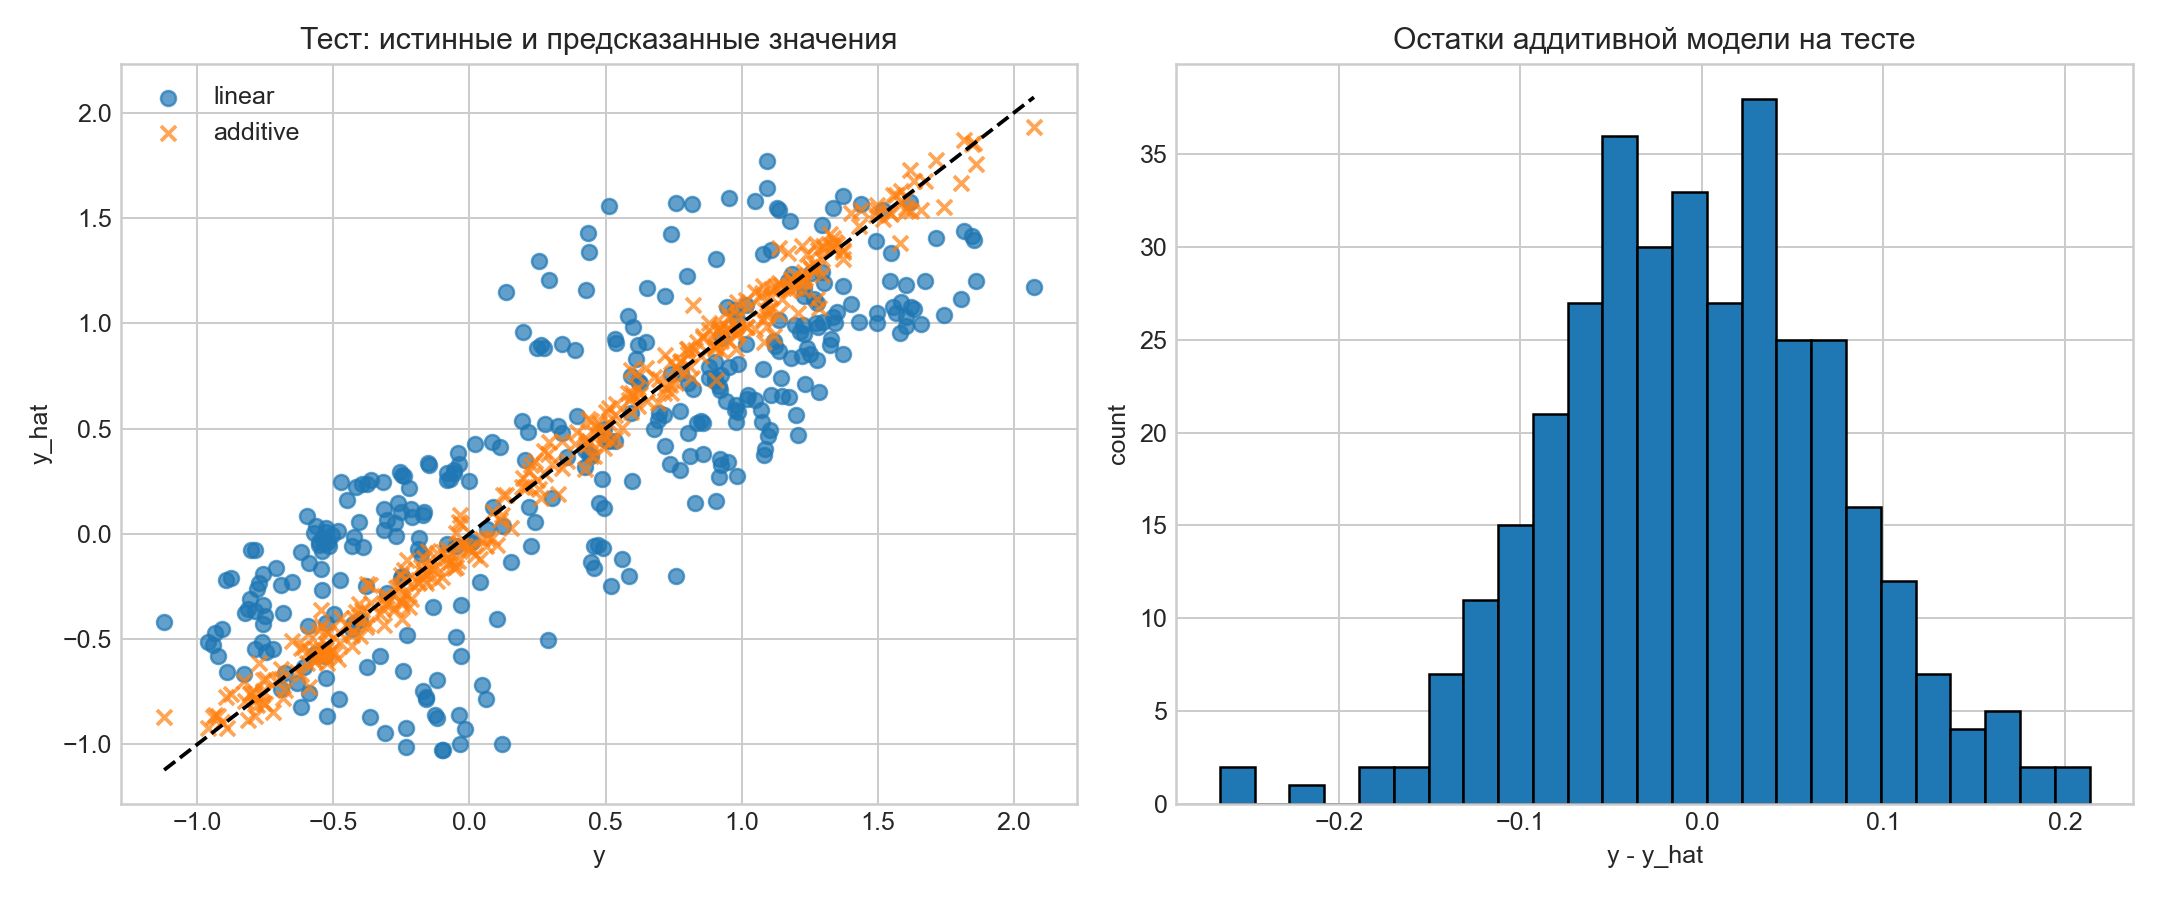
\includegraphics[width=\textwidth]{figures/case7_predictions_and_residuals.png}
    \caption{Предсказания и остатки аддитивной модели на тестовой выборке.}
    \label{fig:case7-pred}
\end{figure}

На рисунке~\ref{fig:case7-pred} предсказания аддитивной модели лежат близко к
диагонали, а остатки не демонстрируют заметного систематического смещения.

\begin{table}[H]
    \centering
    \small
    \caption{Влияние числа базисных функций на качество аддитивной модели.}
    \label{tab:add-m}
    \begin{tabularx}{0.86\textwidth}{c c c c}
        \toprule
        \(M\) &
        \makecell{число\\параметров} &
        \makecell{test RMSE\\(ед. \(y\))} &
        \makecell{test \(R^2\)\\(безразм.)} \\
        \midrule
        1  & 4  & 0.4530 & 0.6456 \\
        3  & 10 & 0.1032 & 0.9816 \\
        5  & 16 & 0.0777 & 0.9896 \\
        8  & 25 & 0.0772 & 0.9897 \\
        10 & 31 & 0.0775 & 0.9896 \\
        15 & 46 & 0.0781 & 0.9895 \\
        \bottomrule
    \end{tabularx}
\end{table}

\begin{figure}[H]
    \centering
    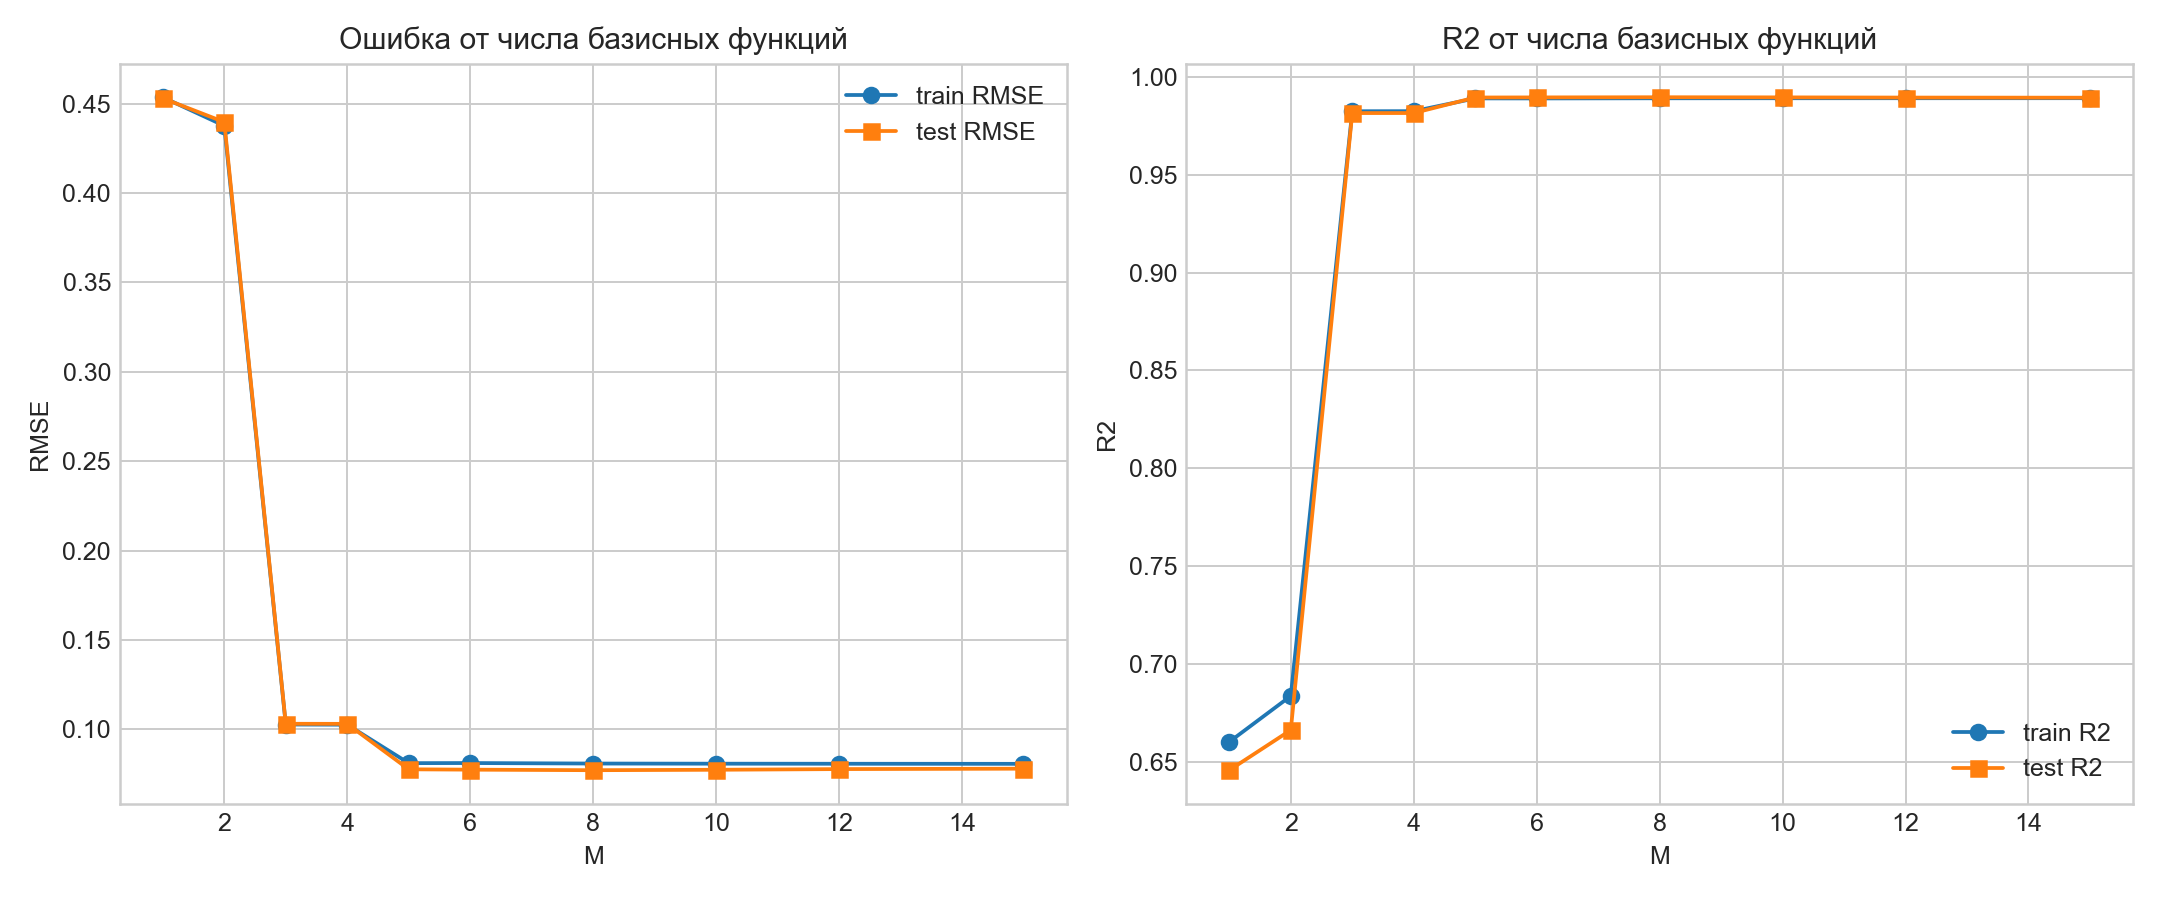
\includegraphics[width=\textwidth]{figures/case7_M_sweep.png}
    \caption{Зависимость качества аддитивной модели от числа базисных функций.}
    \label{fig:case7-m}
\end{figure}

После \(M=5\) тестовая ошибка почти не улучшается. Поэтому дальнейшее
увеличение числа базисных функций не дает существенного выигрыша, хотя
увеличивает число параметров.

\begin{figure}[H]
    \centering
    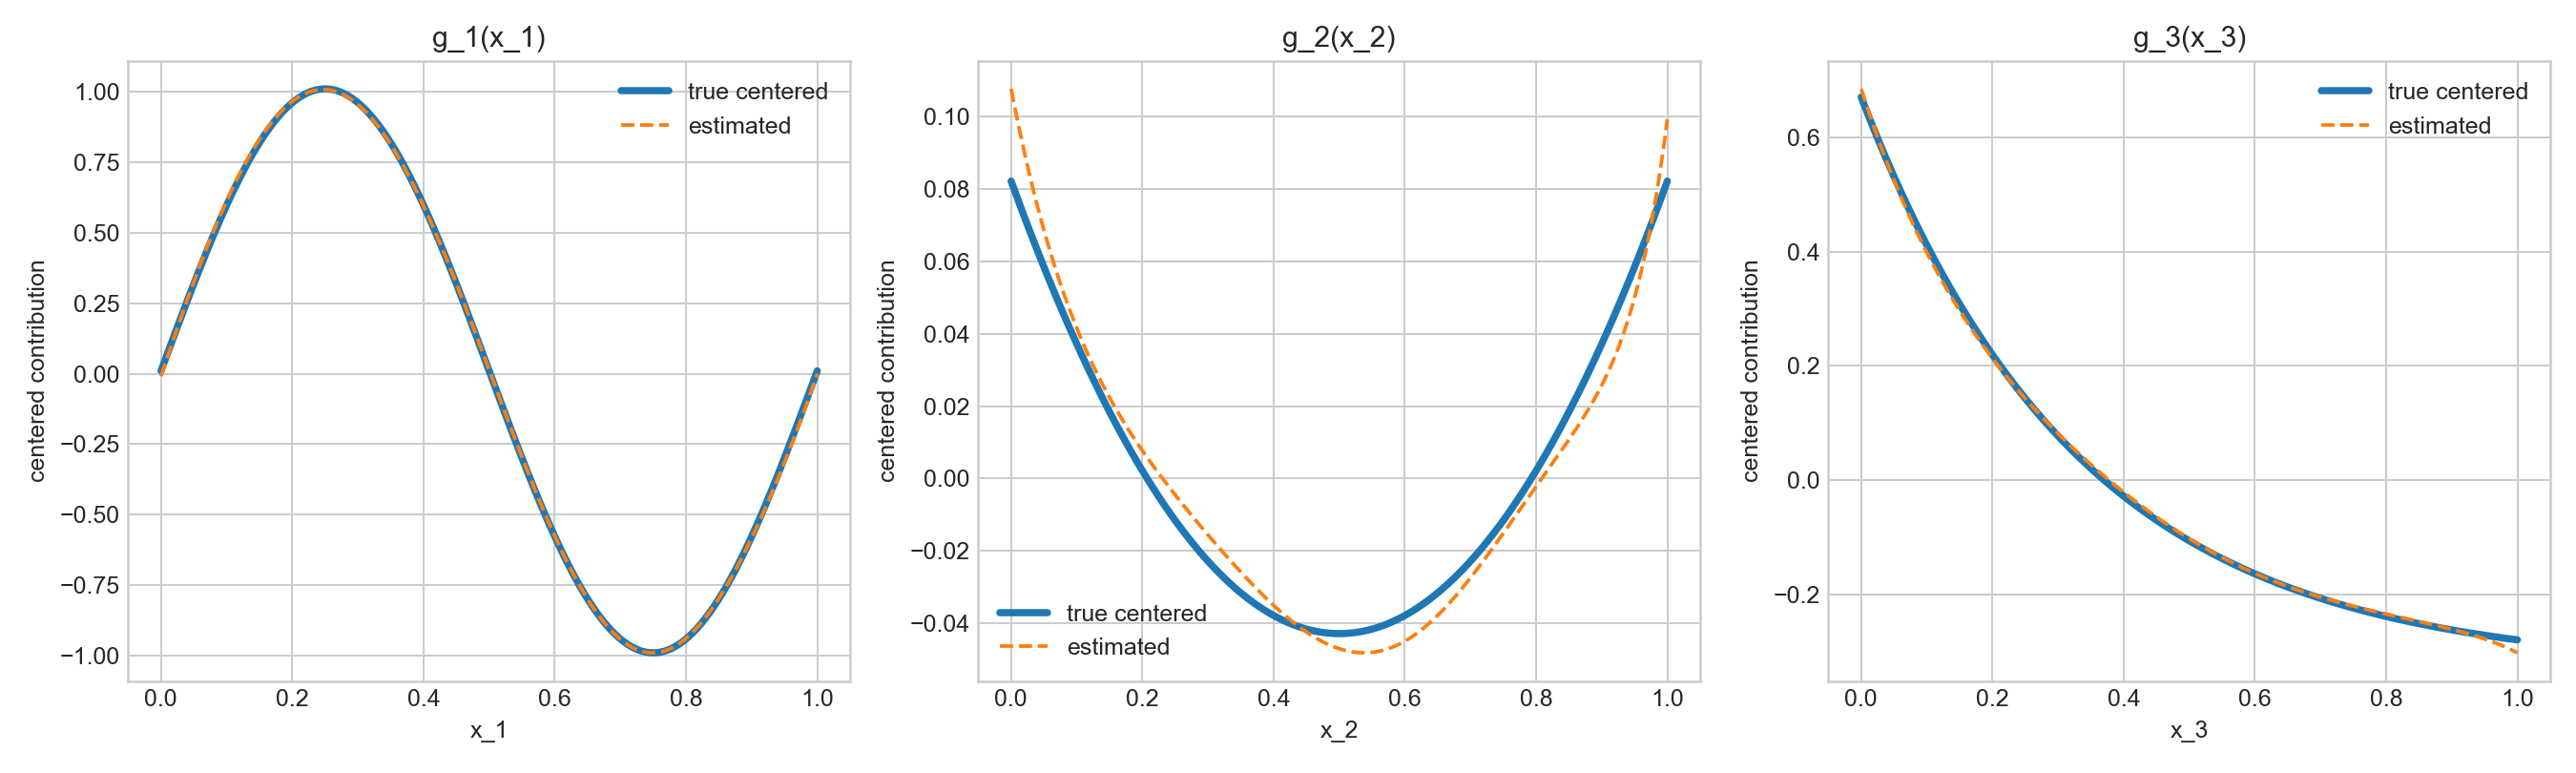
\includegraphics[width=\textwidth]{figures/case7_recovered_components.png}
    \caption{Восстановленные центрированные компоненты \(\widehat g_j\) и
    истинные компоненты на синтетических данных.}
    \label{fig:case7-components}
\end{figure}

Рисунок~\ref{fig:case7-components} показывает, что модель восстанавливает форму
одномерных вкладов. Это важное преимущество аддитивной модели: она дает не
только прогноз, но и интерпретируемое разложение по признакам.

\begin{table}[H]
    \centering
    \small
    \caption{Сравнение аддитивной и полной полиномиальной модели на аддитивных данных.}
    \label{tab:add-full}
    \begin{tabularx}{0.92\textwidth}{X c c c}
        \toprule
        модель &
        \makecell{число\\параметров} &
        \makecell{test RMSE\\(ед. \(y\))} &
        \makecell{test \(R^2\)\\(безразм.)} \\
        \midrule
        additive, \(M=10\) & 31 & 0.0775 & 0.9896 \\
        full polynomial, degree 5 & 56 & 0.0787 & 0.9893 \\
        \bottomrule
    \end{tabularx}
\end{table}

На аддитивных данных полная модель с взаимодействиями не улучшает качество
по сравнению с аддитивной. Это показывает, что более сложная модель не всегда
лучше: если структура данных аддитивна, ограничения модели помогают сохранить
интерпретируемость без потери точности.

Для проверки границ метода рассмотрена неаддитивная зависимость
\[
    y=\sin(2\pi(x_1+x_2))+0.5x_3+\eps.
\]
Здесь признаки \(x_1\) и \(x_2\) входят совместно, поэтому сумма отдельных
функций \(g_1(x_1)+g_2(x_2)\) не обязана хорошо описывать зависимость.

\begin{table}[H]
    \centering
    \small
    \caption{Качество моделей на данных с взаимодействием признаков.}
    \label{tab:nonadd}
    \begin{tabularx}{0.92\textwidth}{X c c c}
        \toprule
        модель &
        \makecell{число\\параметров} &
        \makecell{test RMSE\\(ед. \(y\))} &
        \makecell{test \(R^2\)\\(безразм.)} \\
        \midrule
        linear & 4 & 0.7056 & 0.0311 \\
        additive, \(M=10\) & 31 & 0.7063 & 0.0293 \\
        full polynomial, degree 5 & 56 & 0.1756 & 0.9400 \\
        \bottomrule
    \end{tabularx}
\end{table}

\begin{figure}[H]
    \centering
    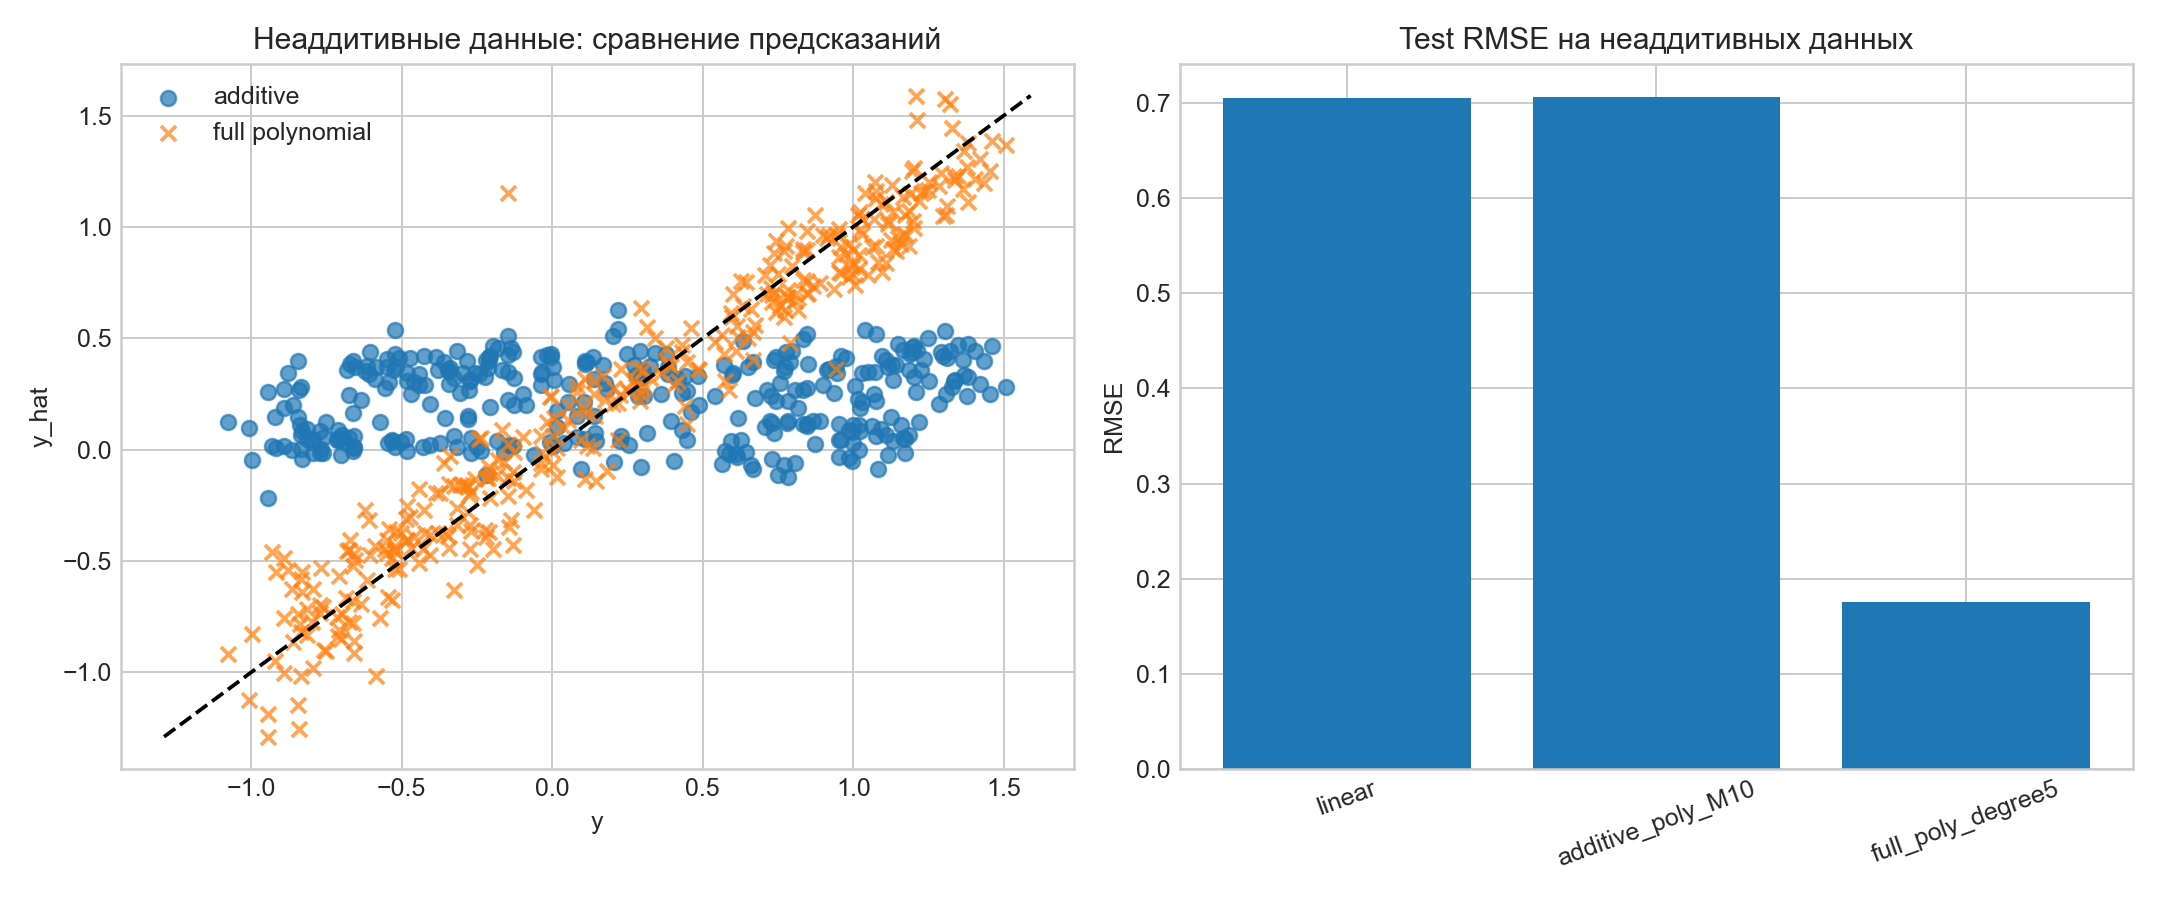
\includegraphics[width=\textwidth]{figures/case7_nonadditive_comparison.png}
    \caption{Сравнение моделей на неаддитивных данных. Модель с взаимодействиями
    заметно лучше аддитивной.}
    \label{fig:case7-nonadd}
\end{figure}

Таблица~\ref{tab:nonadd} и рисунок~\ref{fig:case7-nonadd} показывают, что на
неаддитивных данных аддитивная модель почти не превосходит линейную. Полная
полиномиальная модель выигрывает за счет смешанных признаков, которые позволяют
описать взаимодействие \(x_1+x_2\).

\section{Обсуждение}

В кейсе 3 восстановление становится точным при размерности \(m=3\), что
совпадает с числом положительных собственных значений матрицы Грама. Это
подтверждает связь между рангом матрицы Грама и минимальной размерностью
евклидова вложения. В размерности \(2\) возникает заметная ошибка, потому что
одно существенное направление спектра отброшено.

При добавлении шума матрица расстояний перестает быть точной евклидовой
матрицей: появляются нарушения неравенства треугольника, отрицательные
собственные значения и растущая ошибка восстановления. Поэтому спектр матрицы
Грама является не только способом построить координаты, но и диагностикой
качества исходной матрицы расстояний.

В кейсе 7 аддитивная модель на аддитивных данных достигает test \(R^2=0.9896\)
и заметно превосходит линейную модель, у которой test \(R^2=0.6456\). При этом
более сложная полная полиномиальная модель не улучшает результат на аддитивных
данных, что показывает пользу структурного ограничения.

На неаддитивных данных аддитивная модель почти не превосходит линейную, а
полная модель с взаимодействиями достигает test \(R^2=0.9400\). Это показывает
границу применимости аддитивного подхода: он хорошо работает для суммы
одномерных эффектов, но не описывает совместные зависимости признаков.

\section{Выводы}

\begin{enumerate}[label=\arabic*)]
    \item Матрица расстояний может быть исследована через матрицу Грама,
    полученную двойным центрированием.

    \item Положительная часть спектра матрицы Грама задает координаты
    евклидова вложения, а число положительных собственных значений задает
    минимальную размерность.

    \item В синтетическом эксперименте точное восстановление достигается
    в размерности \(3\); двумерная визуализация удобна, но не является
    изометрической.

    \item Шум разрушает точную евклидову структуру и приводит к отрицательным
    собственным значениям матрицы Грама.

    \item Аддитивная модель существенно лучше линейной на аддитивных
    нелинейных данных и дает интерпретируемые графики вкладов признаков.

    \item Увеличение числа базисных функций полезно только до стабилизации
    тестовой ошибки; дальше растет сложность без существенного выигрыша.

    \item На данных с взаимодействиями признаков нужна более общая модель,
    потому что аддитивная структура становится слишком ограничительной.
\end{enumerate}

\section{Воспроизводимость и использование кода}

Код не вставляется в отчет, поскольку листинг должен быть вынесен в отдельный
проект или ноутбук. Вычисления, таблицы и графики выполнены в Python 3.11+
с помощью скрипта \texttt{src/run\_experiments.py}. Полученные графики
сохранены в папке \texttt{figures}, а таблицы --- в папке \texttt{results}.
Ссылка на проект:
\[
    \CodeRepository
\]

\begin{thebibliography}{9}
\begingroup
\RaggedRight

\bibitem{kolmogorov-fomin}
Колмогоров~А.\,Н., Фомин~С.\,В.
\textit{Элементы теории функций и функционального анализа}.
Москва: Наука, 1976.

\bibitem{kolmogorov1957}
Колмогоров~А.\,Н.
О представлении непрерывных функций нескольких переменных суперпозициями
непрерывных функций одного переменного и сложением.
\textit{Доклады Академии наук СССР}, 114(5), 1957.

\bibitem{torgerson1952}
Torgerson~W.\,S.
Multidimensional scaling: I. Theory and method.
\textit{Psychometrika}, 17, 401--419, 1952.

\bibitem{gower1966}
Gower~J.\,C.
Some distance properties of latent root and vector methods used in multivariate analysis.
\textit{Biometrika}, 53(3--4), 325--338, 1966.

\bibitem{hastie-tibshirani1990}
Hastie~T., Tibshirani~R.
\textit{Generalized Additive Models}.
London: Chapman and Hall, 1990.

\bibitem{esl}
Hastie~T., Tibshirani~R., Friedman~J.
\textit{The Elements of Statistical Learning}.
2nd ed. New York: Springer, 2009.

\bibitem{vorontsov}
Воронцов~К.\,В.
\textit{Математические методы обучения по прецедентам}.
Курс лекций.

\endgroup
\end{thebibliography}

\end{document}
